\chapter{Umsetzung des Prototyps}
Nachdem in Kapitel \ref{sec:concept} die Konzeption der Anwendung vorgestellt wurde kann, kann nun die Umsetzung der Anwendungen erfolgen.

Zunächst wird dabei auf die Ausgangssituation aus dem vorangegangenem Projekt vorgestellt. Im Anschluss erfolgt eine Auflistung der verwendeten Technologien. Danach erfolgt die Vorstellung der Anwendungen, sowie die Herausforderungen und Probleme in der Umsetzung

\section{Ausgangssituation}
In der vorausgehenden Arbeit wurde ein Art \ac{MVP} der Spielidee umgesetzt welche aus 3 Hauptanwendungen bestand. Es gibt eine Unity-Anwendung, in welcher das Spielgeschehen des \say{Players} umgesetzt wurde. Das Spielgeschehen der \say{Watcher}-Anwendung wurde über eine Vue3-Webseite realisiert. Für die Kommunikation der beiden Anwendungen untereinander wurde auf der Basis eines \say{Express.js} Node-Servers ein WebSocket-Server entwickelt. Der Node-WebSocket-Server kommuniziert zusätzlich mit einer MongoDB Datenbank, in welcher die Fortschritte der einzelnen Sessions gespeichert werden.

Die Anwendungen des \say{Players} und des \say{Watchers} sind in dieser Konstellation jeweils Anzeigende und auf die Eingaben des Nutzers reagierende Komponenten im gesamten System. Sie geben eine Rückmeldung an den Server, der die Daten zur Laufzeit abspeichert und persistent in einer Datenbank speichern kann.

\subsection{Aufbau der Ausgangssituation}

Im Softwaredesign wird dabei von einem \ac{MVC} Design-Pattern gesprochen (vgl. \cite{GlossarWiki:Reenskaug:1979a}). 
Das Model definiert, welche Daten die App enthalten soll. Ändert sich der Zustand dieser Daten, informiert das Modell die einzelnen Views, damit die Ansicht der Daten entsprechend aktualisiert werden können. Außerdem wird manchmal auch der Controller über Änderungen informiert. Die View definiert wie die Daten angezeigt werden sollen. Der Controller verarbeitet die reinkommenden Änderungen aus den Views, die die Nutzer getätigt haben, und gibt diese an das Model oder die Views direkt weiter (vgl. \cite{noauthor_mvc_2023}); (vgl. Abbildung \ref{fig:mvc-diagramm}).

\begin{figure}[ht]
\centering
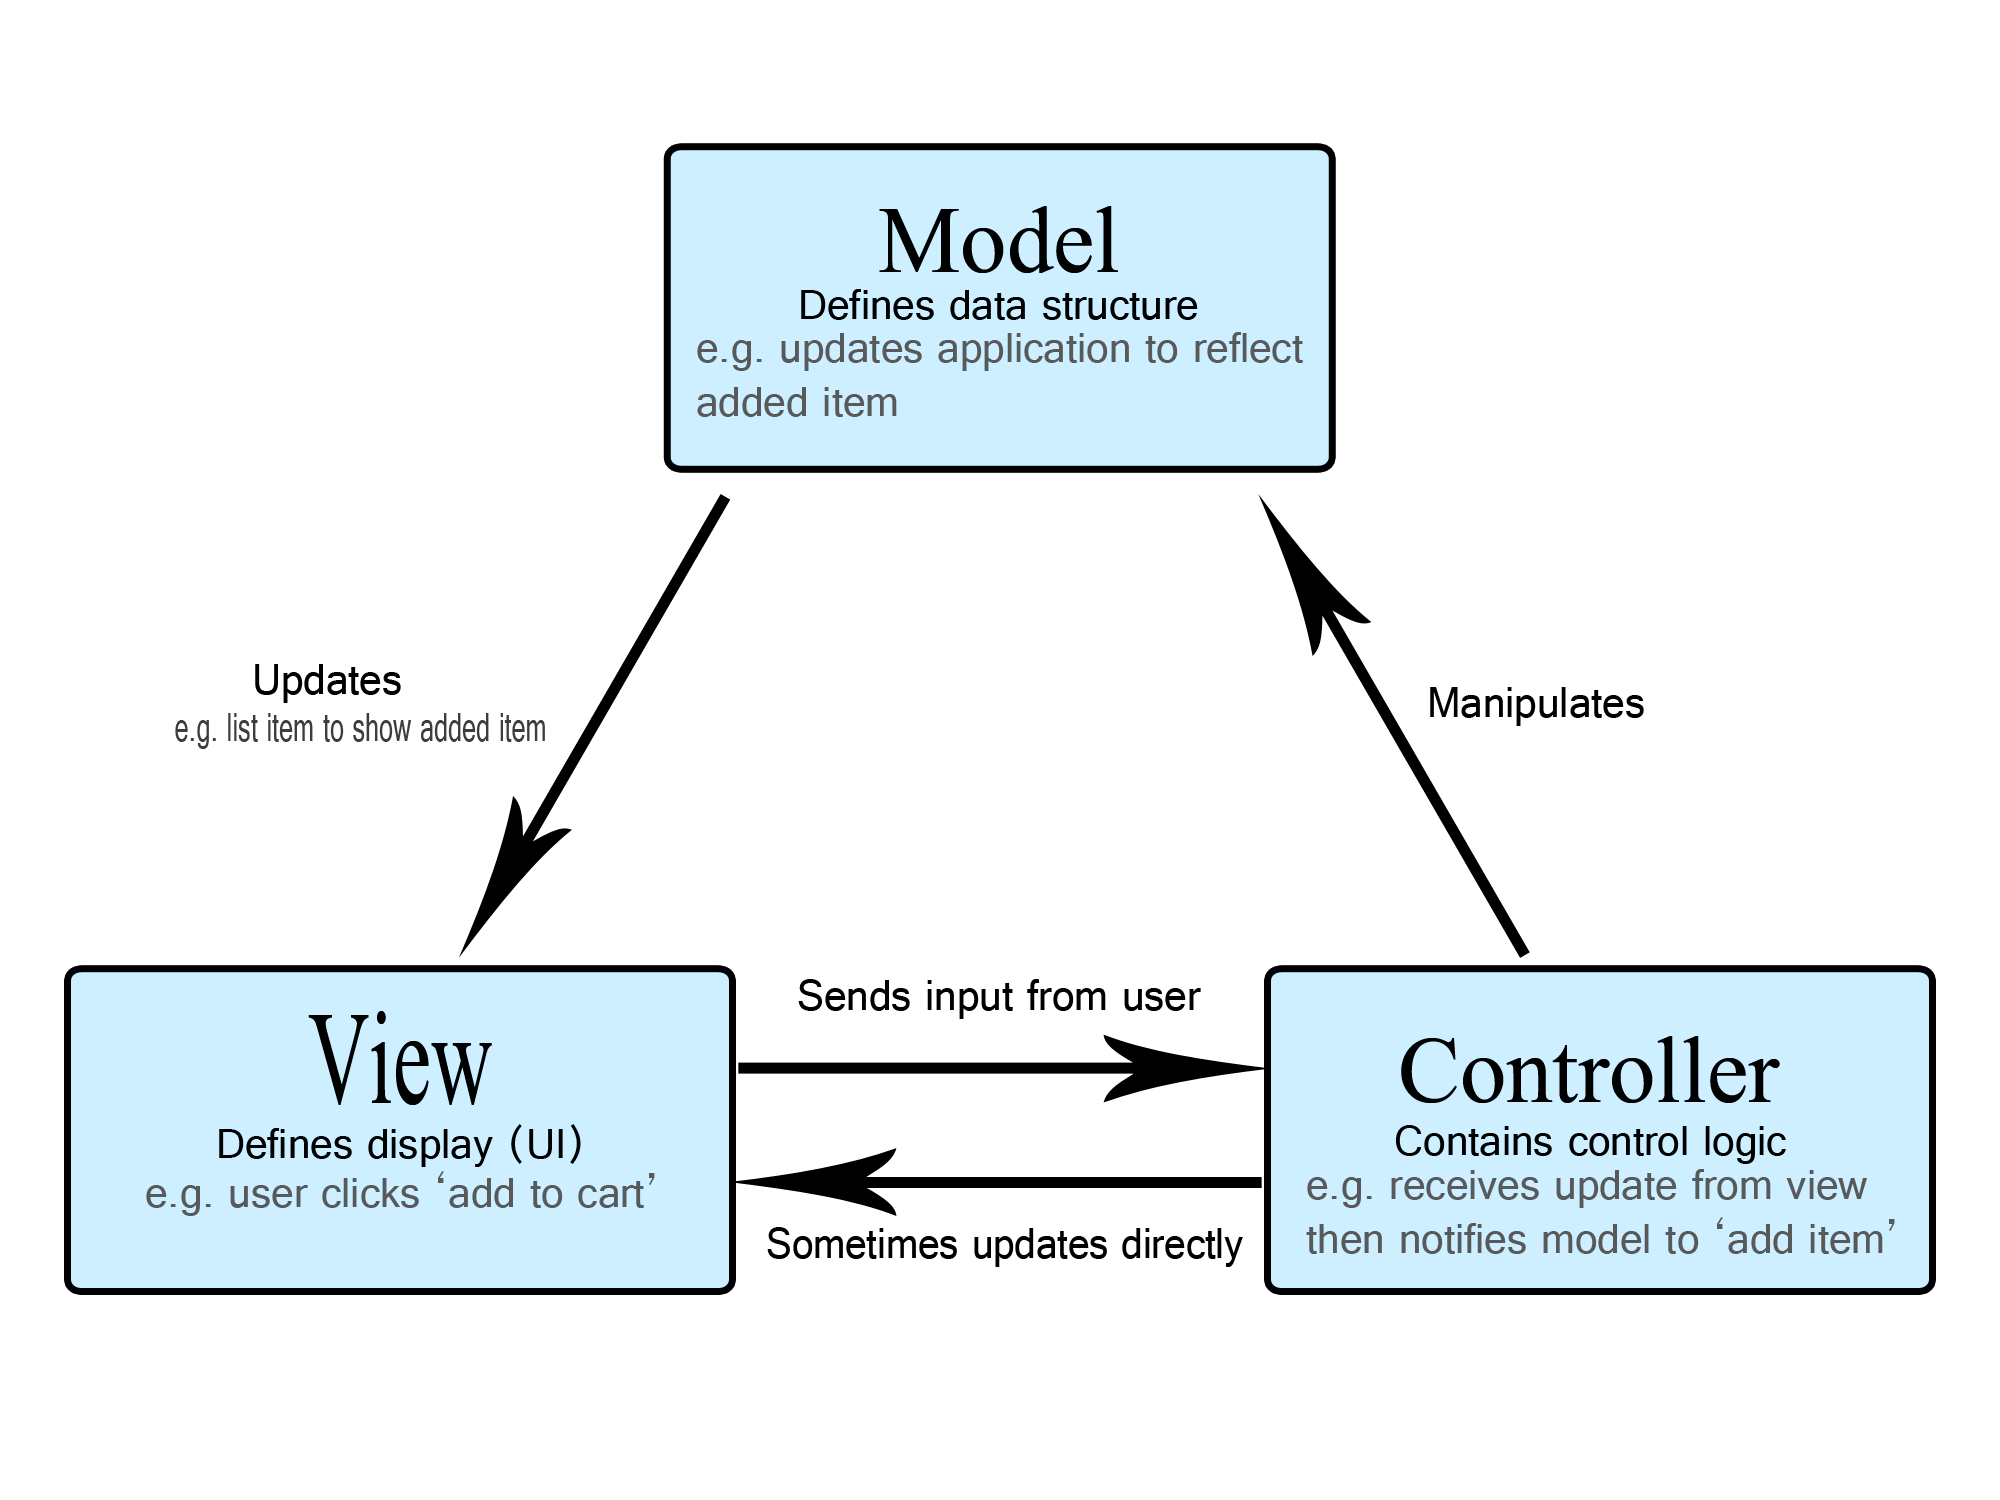
\includegraphics[width=1\linewidth]{content/pictures/mvc-architecture.png}
\caption{\ac{MVC} Beispiel-Diagramm \cite{noauthor_mvc_2023}}
\label{fig:mvc-diagramm}
\end{figure}

Die MongoDB Datenbank und Klassen innerhalb des WebSocket-Servers nehmen die Rolle des Model ein, die einzelnen WebSocket-Nachricht Endpunkte übernehmen die Aufgaben des Controllers und die Anwendung des \say{Watchers} und des \say{Players} sind die Views der Architektur.

\subsection{Beitreten einer Session}

\begin{figure}[ht]
\centering
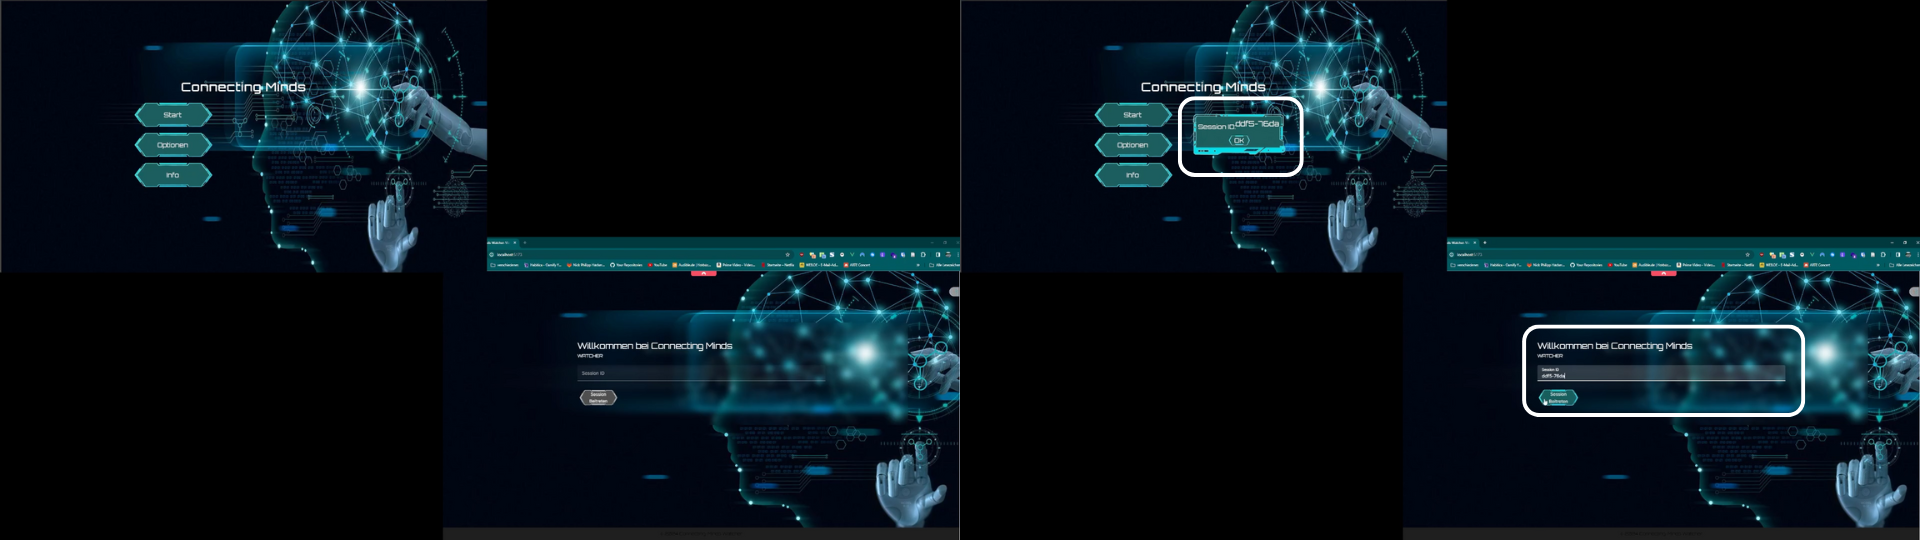
\includegraphics[width=1\linewidth]{content/pictures/Login_Login_by_ID.png}
\caption{Startbildschirme der Player und Watcher Anwendung (Quelle: eigene Darstellung)}
\label{fig:old-logins}
\end{figure}

Abbildung \ref{fig:old-logins} zeigt den bereits im alten Prototyp entwickelten Startbildschirm über welchen der Player eine neue Session starten (linkes Bild, links oben) und der Watcher dieser beitreten kann (linkes Bild, rechts unten). Sobald der Player eine Session erstellt hat, erhält er vom WebSocket-Server eine Rückmeldung mit der erstellten Session-ID (rechtes Bild, links oben) welches er dem Watcher mitteilen muss, damit dieser ihr beitreten kann (rechts Bild, rechts unten).

\subsection{Einführung in die Anwendungen}

\begin{figure}[ht]
\centering
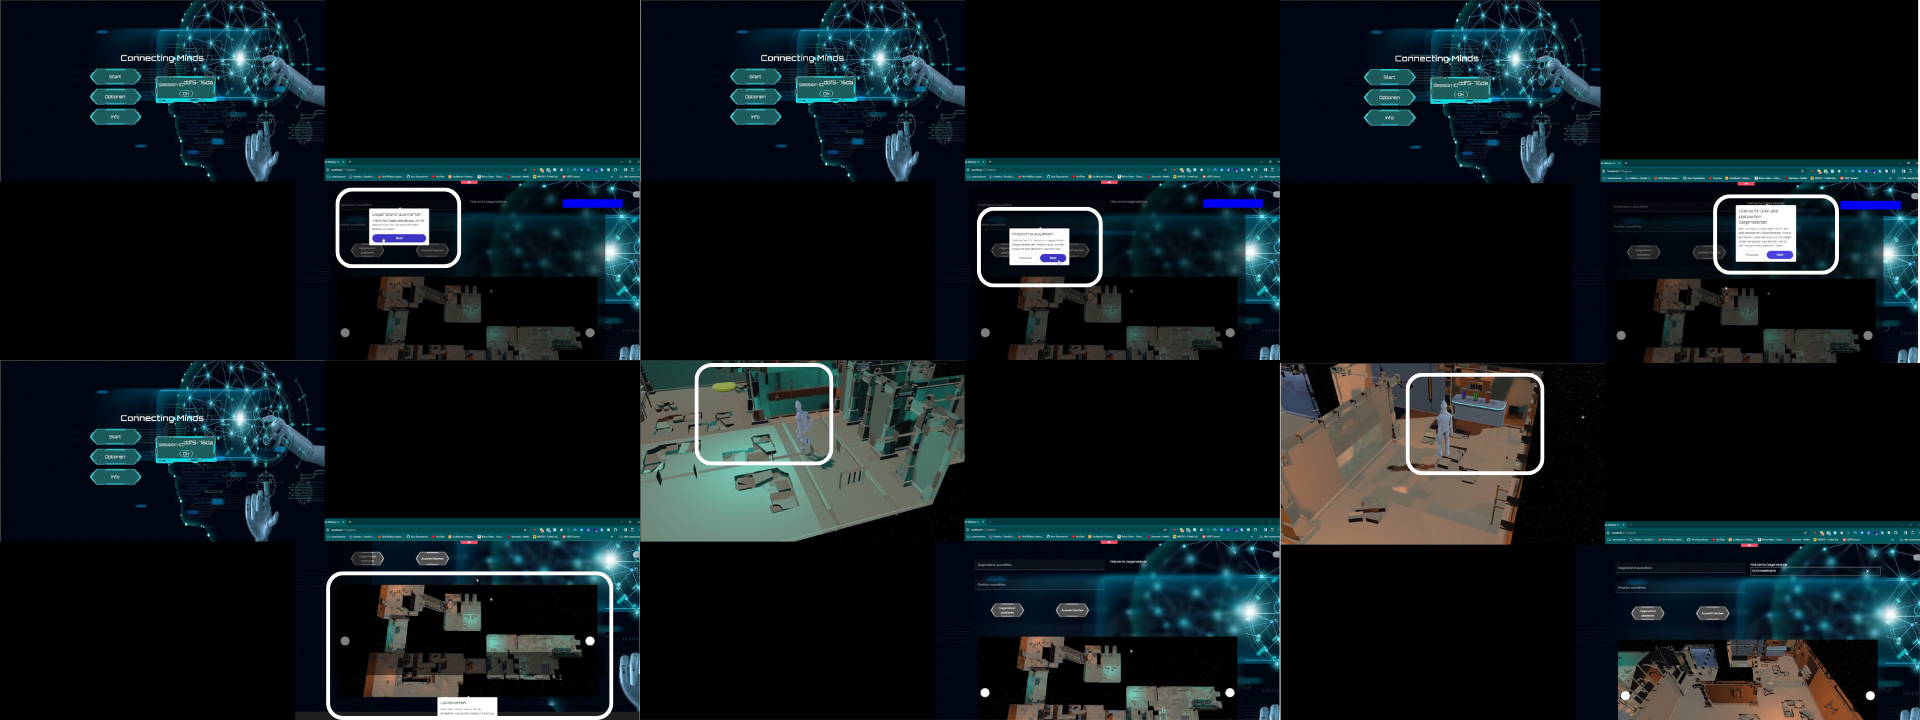
\includegraphics[width=1\linewidth]{content/pictures/Introduction.png}
\caption{Einführung in die Anwendung des Players und Watchers (Quelle: eigene Darstellung)}
\label{fig:old-introductions}
\end{figure}

Abbildung \ref{fig:old-introductions} zeigt die Einführung der beiden Anwendungen in die Spielwelt. Zum Start erhielt der Watcher einzelne Tooltips, mit Erklärungen zu den Grundfunktionen seiner Anwendung (erstes bis drittes Bild in der ersten Zeile und linkes Bild in der zweiten Zeile; jeweils in weiß umrandet im rechten Bildelement). Seine Anwendung enthalten zwei Dropdown-Menüs, über die Gegenstände und Positionen ausgewählt werden können, (erste Zeile, Bilder links und und in der Mitte) eine Liste mit allen platzierten Gegenstände (erste Zeile rechts Bild), die jeweils einzeln entfernt werden können und eine Top-Down-Ansicht der Spielwelt, in der sich der Player befindet (zweite Zeile, linkes Bild). 

Der Player steuert seinen Avatar über eine Touch-druck auf die Spielwelt (zweite Reihe mittlere Bild, linkes Bildelement). Außerdem kann er über vertikale Swipes die Höher der Kamera zum Avatar verändern und dadurch in einem gewissen Rahmen die Ansicht verändern.

Um in der Spielwelt an das Ziel zu gelangen, müssen der Player und Watcher zusammenarbeiten und Hindernisse in der Spielwelt beseitigen. Im linken Bild in der zweiten Zeile im weiß umrandeten wird ein solches Rätselelement dargestellt, welches gelöst werden muss.
\subsection{Lösen von Rätseln}
Wie wurden im alten Prototyp die einzelnen Rätsel gelöst und durch wen erfolgte dies?

\begin{figure}[ht]
\centering
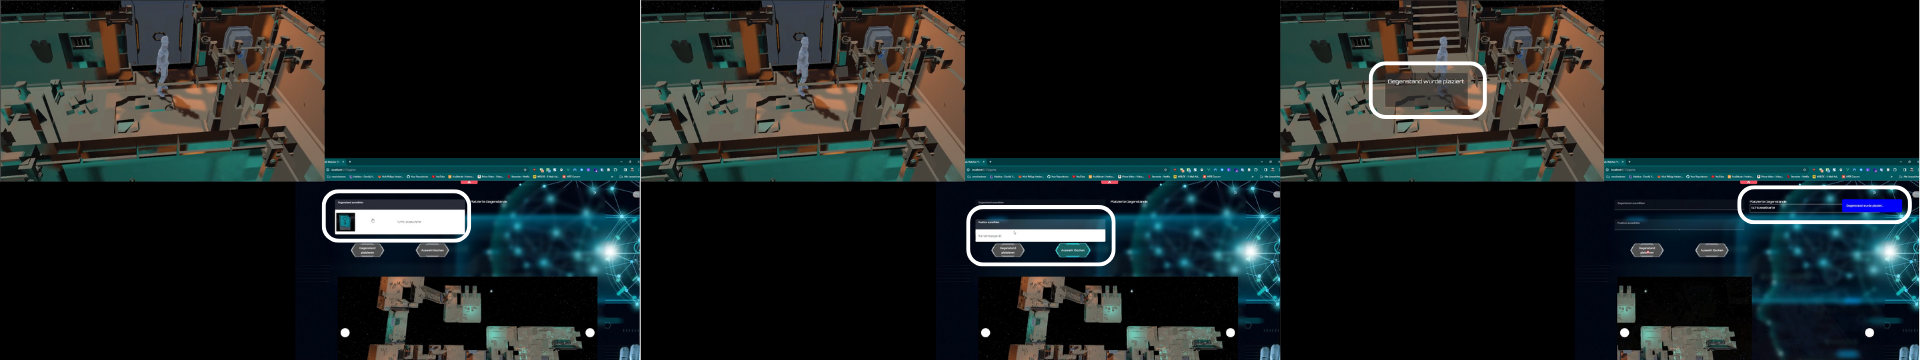
\includegraphics[width=1\linewidth]{content/pictures/HowToSolve.png}
\caption{Vorgang des Lösens von Rätseln (Quelle: eigene Darstellung)}
\label{fig:old-solving-riddle}
\end{figure}

Der Watcher war dafür verantwortlich, dass Gegenstände auf ihre richtigen Zielpositionen platziert wurden. Sobald der Player auf eine Absperrung in der Spielwelt stieß, musste er beschreiben was er sah um dem Watcher einen Hinweis darauf zu geben, welche Gegenstände platziert werden müssen und auf welche Positionen diese gehören. Zunächst wählt der Watcher über das Gegenstände-Dropdown einen entsprechenden Gegenstand aus (linkes Bild, rechtes Bildelement). Anschließend wählt er eine vorgegebene Position aus, die im derzeitig aktiven Abschnitt der Spielwelt hinzugekommen ist (mittlere Bild, rechts Bildelement). Über den Button \say{Gegenstand platzieren} (linker Button) wird der Gegenstand in die Spielwelt des Players platziert. Sowohl der Player als auch der Watcher erhalten vom System eine Benachrichtigung, dass der Gegenstand platziert wurde (rechts Bild, beide weißen Umrandungen). Auf der rechten Seite der Watcher-Anwendung erscheint zur selben Zeit wie die Benachrichtigung der platzierte Gegenstand in der Liste der platzierten Gegenstände (rechtes Bild, rechtes Bildelement). 

\subsection{Freischalten von Gegenständen und Positionen}
Sobald ein Rätsel durch das Platzieren von Gegenständen gelöst wurde, erhielten Player und Watcher die Information, dass neue Gegenstände freigeschaltet wurden (vgl. Abbildung \ref{fig:old-unlock-system}, erste Reihe linkes Bild, eingekreist in weiß). 

\begin{figure}[ht]
\centering
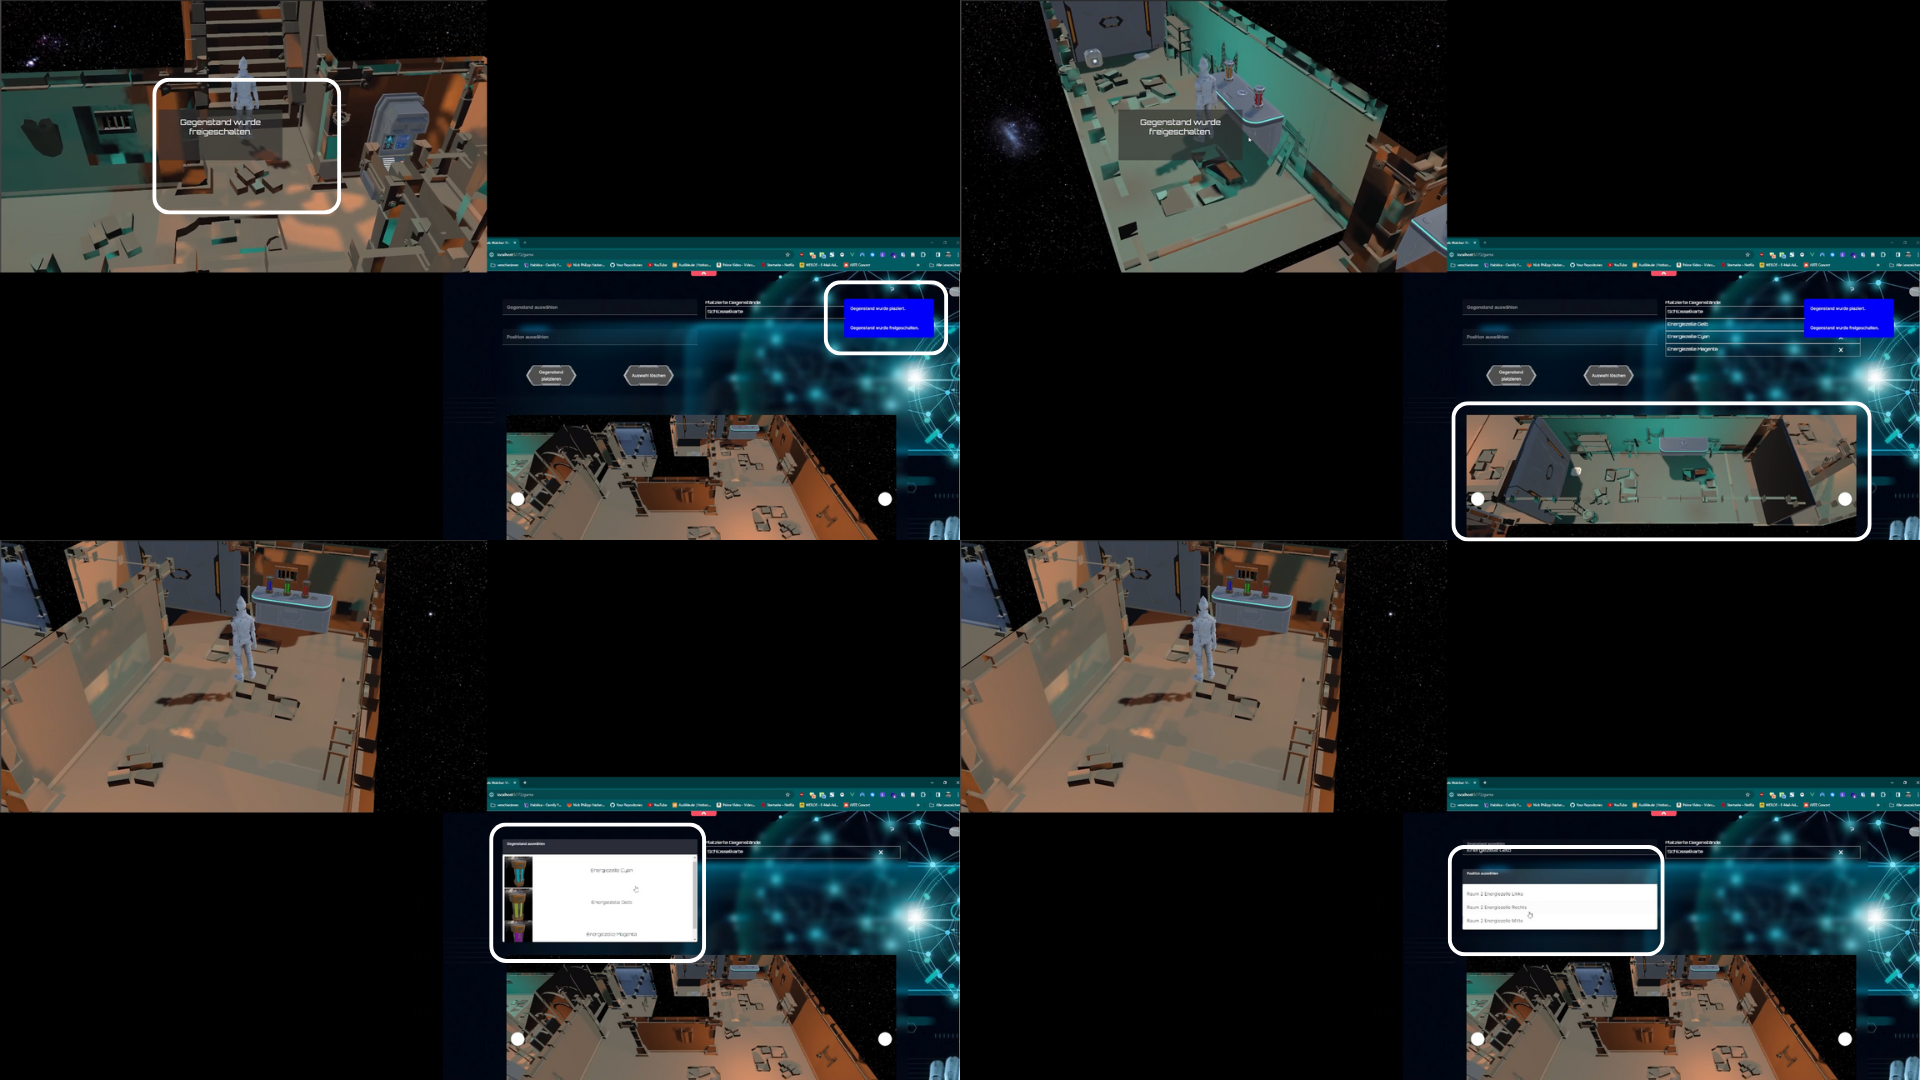
\includegraphics[width=1\linewidth]{content/pictures/UnlockMore.png}
\caption{Freischalten neuer Gegenstände (Quelle: eigene Darstellung)}
\label{fig:old-unlock-system}
\end{figure}

Sobald das Lösen des Rätsel das Hindernis beseitigt und einen neuen Bereich zugänglich macht, geht der Bilder-Slider in der Anwendung des Watchers auf das aktuelle Bild. Der Slider zeigt dem Watcher alle verfügbaren Abschnitte der Spielwelt (vgl. erste Reihe, rechtes Bild, in weiß umrandet in Abbildung \ref{fig:old-unlock-system}). Durch die neuen Spielabschnitte werden nicht nur neue Gegenstände freigeschaltet, sondern auch zusätzliche vordefinierte Positionen, auf denen die Gegenstände platziert werden können. Diese werden dem Watcher in den Gegenstand- und Positions-Dropdown aufgelistet (vgl. Abbildung \ref{fig:old-unlock-system}, beide Bilder in der zweiten Reihe in weiß umrandet). 

\subsection{Aspekte zum Überarbeiten}
% backfaces
% steuerung beim Player

% interaktion mit der spielwelt beim watcher
% feedback von den probandentests aufzählen

\section{Verwendete Technologien}



\section{Aufbau des Prototyps}



\section{Herausforderungen in der Umsetzung}
% erste Ansätze im Levelbuilding erwähnen

% hier kommt das placing also die positionen in der spielwelt

% dann drauf bezogen das mit den slots, dass die ne position haben später auch fürs setzen wichtig
% das mit den collidern, was man auch anders umsetzen kann noch, das noch erwähnen






% bei umsetzung müssen die 3d und ar anwendung vorgestellt werden vom watcher
% hier muss ein bezg auf das paper mit den steuerungen für touch erwähnt werden


% die anwendung vom playewr

\section{Probleme in der Umsetzung}

% AR

% Gerätefindung im selben Netzwerk